% !TEX root = ../main.tex
\section{Problem Statement}
\label{sec:problem}
In most robotic applications, it is important to be able to accurately and reliably calculate the pose of the fiducial tags. There has been large amounts of effort to improve the detection algorithm making them faster and more accurate in the RGB space. The results have been proven to be good under ideal conditions. However, in real robotic application, the algorithm are often ran on a small patch of pixels which causes fundamental problems under different lighting and sensory noise. In fact, we observe that the pose of the tag on a stationary object constantly flickers depending on the lighting. The biggest problem in square tags is introduced by the perceptual ambiguity caused by the perspective projection. In any square fiducial tag detection, the four corners are extracted from the tag and the pose of the tag is estimated using some 3D to 2D point correspondence optimization. However, when the tag is small, small variance in the corner detection process will yield estimations far from the true pose. 

We will illistrate this effect by using two over lapping cubes in figure 3. The marked face of both cubes are interlaced and oriented off by 120 degrees. However, due to projection the squares spears to overlap with small differences. This difference is reflected by the perspective projection where, in theory, the square should only produce one unique pose in 3D space. However, due to sensory noise, lighting noise, image resolution, and other factors,the corners are not perfect. When the corners are close, the result of the optimization can return either one of the two solutions. 
\begin{figure}
\centering
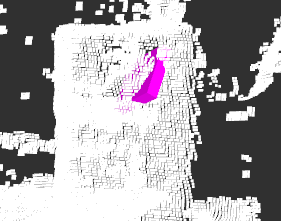
\includegraphics[width=\columnwidth]{figs/mismatch_tag}
\caption{The orientation of Apriltag placed on the object is greatly misaligned with the actual object}
\label{fig:calib}
\end{figure}

\begin{figure}
\centering
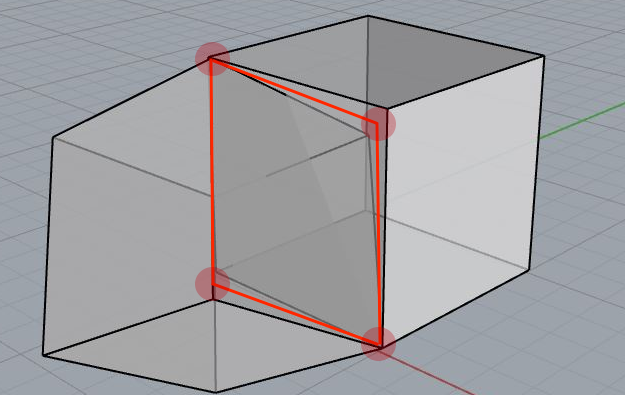
\includegraphics[width=\columnwidth]{figs/perspective_fig}
\caption{Perspective Ambiguity illustrated with overlapping cubes}
\label{fig:calib}
\end{figure}